The dataset of Bitcoin exchange rate to US dollars (BTC-USD) is collected from API of Polygon. The dataset is read in three parts: from 2021/02/20 to 2021/04/25, from 2021/04/26 to 2021/05/26, from 2021/05/27 to 2021/06/27. The frequency is one hour. It total, the collected dataset forms 97 days, which is 2328 hours. 
The date and time were represented in the form of timestamp, which was converted into convenient date-time form. Consequently, the dataset is as follows: \\
\begin{table}[!ht]
\centering
 \begin{tabular}{||c c c c c||} 
 \hline
 Num & Volume & Open & Close & Timestamp \\ [0.5ex] 
 \hline\hline
 1 & 4108.668109 & 55866.00 & 56254.8600 & 2021-02-20 00:00:00\\ 
 2 & 3022.427323 & 56142.00 & 56235.7800 & 2021-02-20 01:00:00\\
 3 & 2126.892304 & 56240.00 & 55741.8800 & 2021-02-20 02:00:00\\
 ... & ... & ... & ... & ... \\
 2328 & 1183.992554 & 38542.80 & 38556.8800 & 2021-05-27 23:00:00 \\ [1ex] 
 \hline
 \end{tabular}
\end{table}

The particular research analyzes and develops the prediction models based on per-hour Close Price data. The graph below represents the Close Price rate over the time:\\
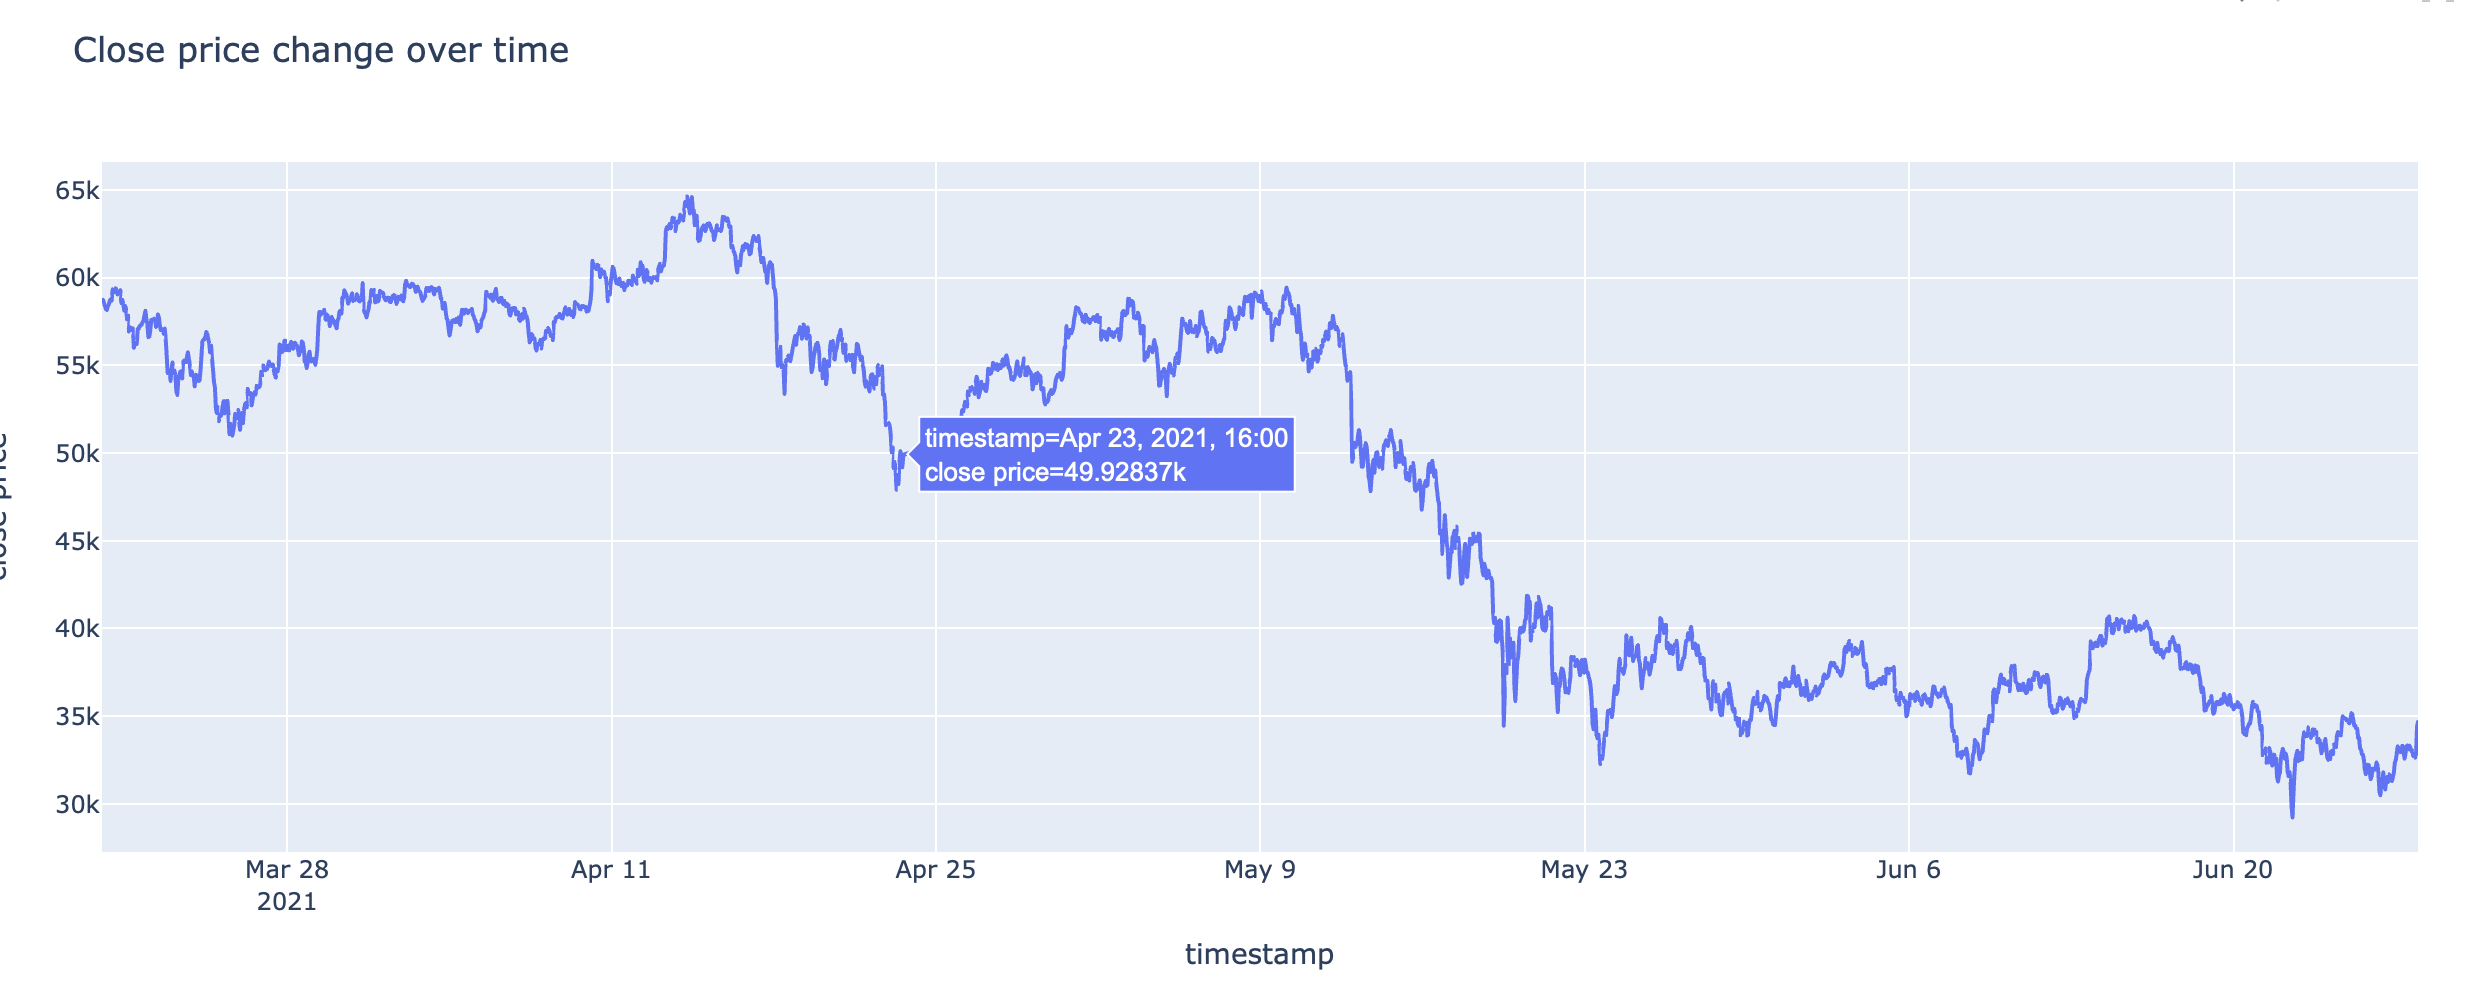
\includegraphics[width=\textwidth]{images/data.png}
Even though the graph above represents that the data is non-stationary, it is necessary to apply an accurate Augmented Dickey-Fuller (ADF) test, which is a statistical test that is built to test whether univariate time series data is stationary or not.

\begin{wrapfigure}{l}{0.25\textwidth}
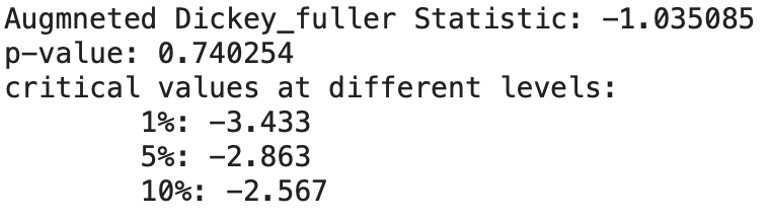
\includegraphics[width=0.9\linewidth]{images/adf.png} 
\label{fig:wrapfig}
\end{wrapfigure}

This test is based on a hypothesis and shows the degree of probability with which it can be accepted. The results obtained suggest that ADF is greater than any critical value at different levels. Moreover, p-value is greater than significance level = 0.05, so there is a fail to reject the null hypothesis H0 at three different confidences: at 90\%, at 95\%, at 99\%. Thus, the data is definitely non-stationary.